\documentclass[11pt,a4paper]{article}

% ---------------------------------------------------------------------------
% Shared NADPH regeneration sets sharp limits on joint glutathione and
% thioredoxin service.
%
% Author metadata: set the macros below before submission.  They are
% deliberately left blank in this version.
% ---------------------------------------------------------------------------
\newcommand{\PaperAuthor}{}
\newcommand{\PaperAffiliation}{}
\newcommand{\PaperDate}{16 September 2026}
\newcommand{\RepositoryNote}{The repository location will be supplied with the author information.}

\usepackage[T1]{fontenc}
\usepackage[utf8]{inputenc}
\usepackage{lmodern}
\usepackage{microtype}
\usepackage[a4paper,margin=1.05in]{geometry}
\usepackage{amsmath,amssymb,amsthm,mathtools}
\usepackage{booktabs}
\usepackage{array}
\usepackage{enumitem}
\usepackage{xcolor}
\usepackage{graphicx}
\usepackage{capt-of}
\usepackage{tikz}
\usetikzlibrary{arrows.meta,positioning}
\usepackage[obeyspaces,spaces]{url}
\usepackage[numbers,sort&compress]{natbib}
\usepackage[colorlinks=true,linkcolor=blue!55!black,citecolor=blue!55!black,urlcolor=blue!55!black]{hyperref}
\hypersetup{pdftitle={Shared NADPH regeneration sets sharp limits on joint glutathione and thioredoxin service},
  pdfkeywords={redox kinetics, NADPH, glutathione peroxidase, peroxiredoxin, thioredoxin,
    resource competition, steady state, monotone response, formal verification, Lean}}

\DeclareUrlCommand\lean{\urlstyle{tt}}
% Typeset bibliography DOIs in text mode so escaped characters render correctly.
\providecommand{\doi}[1]{doi: #1}
\setlist{itemsep=2pt,topsep=3pt}
\setlength{\emergencystretch}{1.5em}
\graphicspath{{figures/}}

\theoremstyle{plain}
\newtheorem{theorem}{Theorem}[section]
\newtheorem{proposition}[theorem]{Proposition}
\newtheorem{lemma}[theorem]{Lemma}
\newtheorem{corollary}[theorem]{Corollary}
\theoremstyle{definition}
\newtheorem{definition}[theorem]{Definition}
\theoremstyle{remark}
\newtheorem{remark}[theorem]{Remark}
\newtheorem{example}[theorem]{Example}

\newcommand{\R}{\mathbb R}
\newcommand{\uM}{\ensuremath{\mu\mathrm{M}}}
\newcommand{\fluxunit}{\ensuremath{\mu\mathrm{M}\,\mathrm{s}^{-1}}}
\newcommand{\dd}{\,\mathrm d}
\newcommand{\Gm}{\Gamma}

\title{\bfseries Shared NADPH regeneration sets sharp limits on\\ joint glutathione and thioredoxin service}
\author{\PaperAuthor\\ \PaperAffiliation}
\date{\PaperDate}

\begin{document}
\maketitle

\begin{abstract}
Two antioxidant branches that operate adequately in separate preparations need not
meet the same branch-resolved requirements when they are coupled to a single NADPH
regeneration system. We study a maintained-peroxide subsystem of published redox
kinetics that retains finite enzyme and carrier inventories, including
enzyme-bound glutathione. Exact elimination of the private states gives, for each
branch, a positive quadratic carrier response and a strictly increasing service
current as a function of the shared NADPH concentration. Against a strictly
decreasing regeneration current this yields a necessary and sufficient condition
for joint service, an explicit and attained minimum regeneration capacity, a
reconstruction of every steady-state species, and uniqueness of the full joint
steady state. We prove that a finite regeneration repair exists exactly when each
quota lies strictly below its branch ceiling current, and we identify the exact
deficit of a quota-only capacity estimate as kinetic overdelivery. For declared
nominal parameters and design quotas of $10$ and $4$ \fluxunit, both isolated
preparations succeed while their joint preparation fails at one tenth of the
reference regeneration capacity; the attained minimum requires a certified
$13.71266$--$13.71268\%$ increase over that setting. Allowing one enzyme
inventory to change attains the quota-only bound exactly, with a $3.3727\%$
reduction in the glutathione peroxidase pool, and we prove a matching lower bound
over every admitted redesign of that branch. The decision criterion, the
separate-preparation comparison, the uniqueness and ceiling theorems and the
constructive redesign are checked in Lean~4. We also delimit the result: we give
the exact interval criterion that replaces the threshold when branch service is
not monotone, an explicit analytic example in which excess regeneration destroys
service without bistability, and a sign obstruction showing that the eight-variable
kinetics admit no orthant order making them cooperative near the boundary
equilibrium. The result concerns kinetic service in a declared maintained system.
It is not a claim about whole-cell protection, clinical benefit, or thermodynamic
incompatibility.
\end{abstract}

\section{Introduction}\label{sec:intro}

Shared reducing power couples reactions that can each look adequate in isolation.
Glutathione peroxidase and the peroxiredoxin--thioredoxin system both clear
hydrogen peroxide, and both are ultimately restored by NADPH through their own
reductases \citep{winterbourn2008,lu2014,sies2017}. A design question that arises
whenever such branches are assembled into one preparation is therefore not merely
whether each branch has sufficient enzyme, but whether the service each branch is
required to deliver can coexist with the other at one physically shared NADPH
concentration.

Answering that question requires actual kinetic demand rather than an assigned
flux. A branch can consume more reducing power than its specified minimum service,
and deleting its requirement does not delete that consumption. This distinction is
the whole content of the difference between the two capacity numbers computed
below, and it is not an artefact of a particular numerical solver.

\citet{adimora2010} developed a coupled model of cellular hydrogen peroxide
responses that includes glutathione, thioredoxin, peroxiredoxin, protein thiols and
catalase. The present contribution is not the introduction of that biochemical
coupling, nor a new calibration of it. It is an exact decision and reconstruction
theorem for a specified maintained subnetwork of those kinetics. The proof retains
the private enzyme and carrier states before eliminating them at steady state, and
identifies precisely which scalar boundary determines joint operation.

\paragraph{Results.}
Let $x$ denote the shared NADPH concentration. After exact elimination, each branch
$i$ has a carrier $u_i(x)$ solving a quadratic with a single positive root and a
service current $j_i(x)$ that is a strictly increasing rational function of $u_i$
(Propositions~\ref{prop:elimination} and~\ref{prop:threshold}). A quota
$j_i\ge q_i$ is therefore equivalent to an explicit NADPH floor $x\ge X_i$. Against
the strictly decreasing regeneration current this gives:

\begin{itemize}
\item a necessary and sufficient criterion for joint service, with an attained
  minimum regeneration scale $s_{\min}=J(L)/R_1(L)$ at $L=\max_iX_i$
  (Theorem~\ref{thm:main});
\item uniqueness of the full joint steady state, in every private enzyme and
  carrier coordinate, not only in $x$ (Theorem~\ref{thm:unique});
\item an exact identity for the deficit of the quota-only capacity estimate,
  namely total kinetic overdelivery at the binding floor
  (Proposition~\ref{prop:overdelivery});
\item an equivalence for repairability: some finite regeneration scale works if and
  only if $q_i<j_i(N)$ for both branches, where $N$ is the largest admissible NADPH
  concentration (Theorem~\ref{thm:ceiling});
\item a constructive change of one enzyme inventory that attains the quota-only
  bound, together with a matching lower bound over all admitted redesigns of that
  branch (Section~\ref{sec:redesign}).
\end{itemize}

Sections~\ref{sec:scope} and~\ref{sec:dynamics} delimit the result rather than
extend it. We record which hypotheses the criterion actually needs, what replaces
it when branch service is not monotone, and exactly what the numerical dynamics do
and do not establish.

\paragraph{What is claimed and what is not.}
Every theorem below is a statement about a declared kinetic system with fixed
peroxide, conserved carrier inventories and an externally maintained regeneration
drive. The service quotas are independently specified design requirements; they are
not measured health thresholds, and we translate them into reduced-carrier floors
so that this is visible. Nothing here establishes whole-cell protection, a clinical
intervention, a thermodynamic impossibility, or global attraction of the full
kinetics. The formal verification described in Appendix~\ref{app:formal}
establishes that the stated propositions follow from their stated hypotheses in
Lean's kernel; it does not validate the choice of equations, the transcription of
the source model, or any biological interpretation.

\paragraph{Organization.}
Section~\ref{sec:model} states the maintained model and what service means.
Section~\ref{sec:boundary} gives the elimination, the criterion and uniqueness.
Section~\ref{sec:consequences} derives design consequences, and
Section~\ref{sec:redesign} the optimal enzyme reallocation.
Section~\ref{sec:nominal} works the nominal preparation.
Section~\ref{sec:scope} determines how far the criterion extends,
Section~\ref{sec:dynamics} treats the full dynamics, and
Section~\ref{sec:relation} compares with existing methods and describes a
discriminating experiment. Appendix~\ref{app:ode} gives the full ODE and the
numerical protocol, Appendix~\ref{app:box} a conservative parameter-box bound, and
Appendix~\ref{app:formal} the formal-verification scope and declaration map.

\section{The maintained model}\label{sec:model}

All concentrations are in \uM\ and time in seconds. The peroxide concentration $H$
is externally fixed, so that the peroxide-dependent rate constants below are
constants of the maintained preparation.

\subsection{Shared pyridine pool and regeneration}

Write $x$ for NADPH and $P-x$ for NADP$^+$, where the pyridine total $P$ is
conserved, and write $P_0$ for the baseline oxidized concentration retained by the
source model's regeneration law. With
\[
  N=P-P_0,\qquad D=K+P,
\]
regeneration is
\begin{equation}\label{eq:source}
  R_s(x)=sV\,\frac{N-x}{D-x}=s\,R_1(x),\qquad 0<x\le N<D,\quad s,V>0 .
\end{equation}
Here $V$ is a reference capacity, $s>0$ is a dimensionless regeneration scale, and
the product $sV$ is a \emph{capacity} parameter. The realized regeneration current
is $R_s(x)$, which is strictly smaller than $sV$ throughout the physical range; we
keep this distinction in every table and figure. The substrate and energy supply
driving this source are maintained, not modelled as a finite reservoir.

Two structural facts about \eqref{eq:source} are all that the argument uses:
$R_s$ is strictly decreasing on $[0,N]$, and $R_s(N)=0$. Section~\ref{sec:general}
records the corresponding general statement.

\subsection{Glutathione branch}

Let $g$ and $z$ denote free GSH and GSSG, and let $e_0,e_1,e_2$ denote reduced
GPx, oxidized GPx and the GPx--SSG intermediate. With branch-specific positive
constants $a_G,b_G,c_G,k_G$ the four currents are
\begin{equation}\label{eq:gcurrents}
  a_Ge_0,\qquad b_G\,g\,e_1,\qquad c_G\,g\,e_2,\qquad k_G\,x\,(z-z_{G0}),
\end{equation}
the last being the baseline-corrected glutathione reductase law. The maintained
peroxide concentration is absorbed into $a_G$. At steady state all four currents
equal a common value $j_G$. The conservation laws are
\begin{equation}\label{eq:gpools}
  e_0+e_1+e_2=E_G,\qquad g+2z+e_2=G .
\end{equation}
The final term of the second law counts the glutathione bound in the enzyme
intermediate. Omitting it gives a different model and a different decision
boundary, even when the intermediate's concentration is numerically small.

\subsection{Peroxiredoxin--thioredoxin branch}

Let $y$ and $z_T$ denote reduced and oxidized Trx, with $y+z_T=T$, and let
$r,h,w,v$ denote reduced, sulfenic, hyperoxidized and disulfide Prx. The
transitions are
\begin{equation}\label{eq:prx}
  r\xrightarrow{\;a_T\;}h,\qquad h\xrightarrow{\;b_T\;}w,\qquad
  w\xrightarrow{\;c_T\;}h,\qquad h\xrightarrow{\;d_T\;}v,\qquad
  v\xrightarrow{\;e_Ty\;}r .
\end{equation}
The peroxide concentration is absorbed into $a_T$ and $b_T$. The transition
$w\to h$ returns hyperoxidized to sulfenic Prx; it is retained exactly as the
source model's first-order phenomenological maintenance law. The model does not
resolve its energetic or reducing inputs, which in biological sulfiredoxin repair
include ATP and a thiol reductant \citep{jonsson2008}; we therefore keep it
visible as an external input throughout (Table~\ref{tab:accounting}). Thioredoxin
regeneration is $k_T\,x\,(z_T-z_{T0})$. At steady state,
\begin{equation}\label{eq:tsteady}
  a_Tr=d_Th=e_Tyv=k_Tx(z_T-z_{T0})=j_T,\qquad c_Tw=b_Th,\qquad r+h+w+v=E_T .
\end{equation}
All rate constants are positive except that $b_T\ge0$ is allowed, and the
baselines $z_{G0},z_{T0}$ are nonnegative.

\subsection{Ownership, service and observables}

\begin{figure}[tb]
\centering
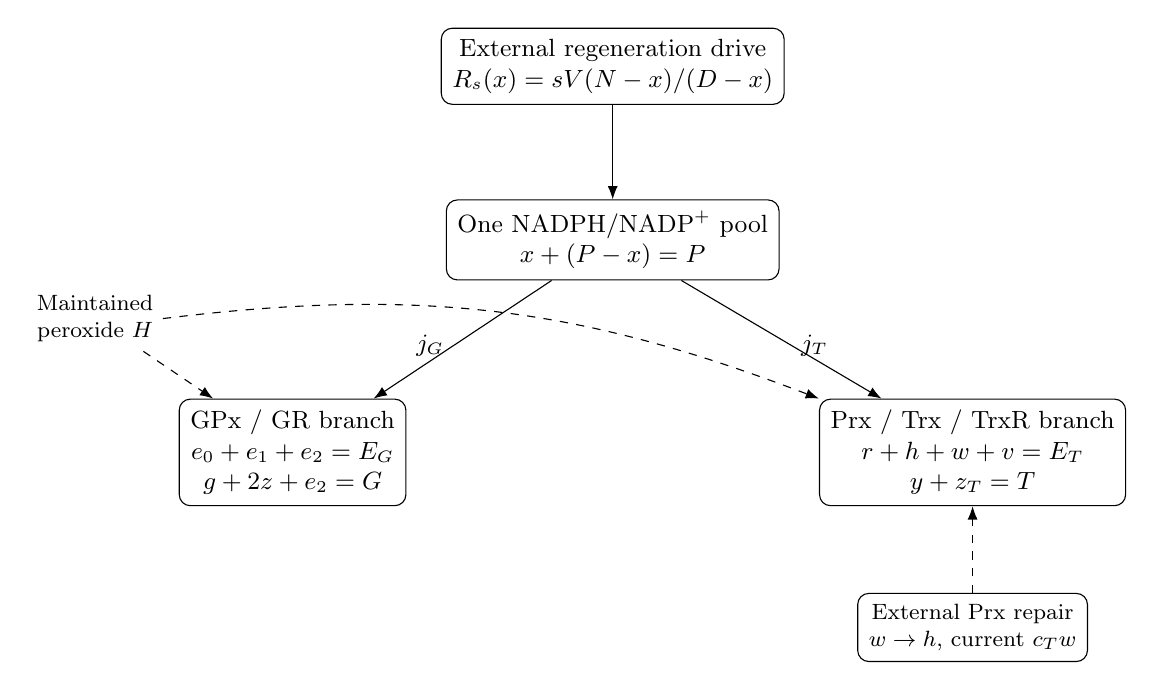
\begin{tikzpicture}[scale=1,>=Latex,node distance=12mm,every node/.style={font=\small},
   box/.style={draw,rounded corners,align=center,inner sep=4pt}]
\node[box] (source) {External regeneration drive\\ $R_s(x)=sV(N-x)/(D-x)$};
\node[box,below=of source] (pool) {One NADPH/NADP$^+$ pool\\ $x+(P-x)=P$};
\node[box,below left=15mm and 5mm of pool] (g) {GPx / GR branch\\ $e_0+e_1+e_2=E_G$\\ $g+2z+e_2=G$};
\node[box,below right=15mm and 5mm of pool] (t) {Prx / Trx / TrxR branch\\ $r+h+w+v=E_T$\\ $y+z_T=T$};
\node[above left=6mm and 2mm of g,align=center,font=\footnotesize] (per) {Maintained\\ peroxide $H$};
\node[box,below=11mm of t,font=\footnotesize] (repair) {External Prx repair\\ $w\to h$, current $c_Tw$};
\draw[->] (source)--(pool);
\draw[->] (pool)--node[left,pos=0.55] {$j_G$} (g);
\draw[->] (pool)--node[right,pos=0.55] {$j_T$} (t);
\draw[->,dashed] (per)--(g);
\draw[->,dashed] (per.east) to[bend left=14] (t.north west);
\draw[->,dashed] (repair)--(t);
\end{tikzpicture}
\caption{Physical ownership in the maintained preparation. The two branches keep
private carrier and enzyme inventories but draw on one NADPH regeneration
balance. Dashed arrows denote externally maintained inputs. The Prx repair
input lies outside the counted NADPH currents, and the peroxide clamp is an
experimental assumption rather than a finite bolus.}
\label{fig:scheme}
\end{figure}

The branches share the variable $x$ and one balance,
\begin{equation}\label{eq:balance}
  R_s(x)=j_G+j_T ,
\end{equation}
and nothing else: enzyme pools, carrier pools and baselines are private
(Figure~\ref{fig:scheme}).

\begin{definition}[Joint service]\label{def:service}
Given quotas $q_G,q_T>0$, \emph{joint service at scale $s$} means the existence of
a steady state of the full system with $0<x\le N$, all private concentrations
positive (with $w=0$ permitted exactly when $b_T=0$), satisfying
\eqref{eq:gpools}, \eqref{eq:tsteady}, \eqref{eq:balance} and
$j_G\ge q_G$, $j_T\ge q_T$.
\end{definition}

The quotas are independently specified assay requirements. Section~\ref{sec:floors}
translates them into equivalent reduced-carrier floors, which is the form in which
they are measurable; they are not measured health thresholds. Two operations that
are often conflated must be separated at the outset:

\begin{itemize}
\item A \emph{separate preparation} physically removes the other branch, and with
  it that branch's demand: the removed term disappears from \eqref{eq:balance}.
\item \emph{Relaxing a quota} removes only an inequality. Both terms remain in
  \eqref{eq:balance}, and the removed branch's kinetic consumption is unchanged.
\end{itemize}

Peroxide removal is a different observable from NADPH consumption. At steady state
GPx removes peroxide at rate $j_G$, while Prx removes it at
$a_Tr+b_Th=j_T(1+b_T/d_T)$, so the maintained peroxide influx that this selected
subsystem requires is
\begin{equation}\label{eq:peroxide}
  I_H=j_G+j_T+\frac{b_T}{d_T}\,j_T ,
\end{equation}
where the last contribution is accompanied by the external repair current $c_Tw$.
Counted NADPH consumption is $j_G+j_T$. No omitted pathway is silently included in
either observable. Away from equilibrium the peroxide sink is instead
$a_Ge_0+a_Tr+b_Th$ and the instantaneous source demand is
$k_Gx(z-z_{G0})+k_Tx(z_T-z_{T0})$; these coincide with the branch service currents
only at steady state.

\section{Exact elimination and the joint boundary}\label{sec:boundary}

Set
\begin{equation}\label{eq:rhos}
  \rho_G=a_G\!\left(\frac1{b_G}+\frac1{c_G}\right),\quad S_G=G-2z_{G0},
  \qquad
  \rho_T=\frac1{a_T}+\frac1{d_T}+\frac{b_T}{c_Td_T},\quad S_T=T-z_{T0},
\end{equation}
and assume throughout the \emph{positive-pool conditions}
\begin{equation}\label{eq:poolcond}
  S_G\rho_G>\frac{E_Ga_G}{c_G},\qquad S_T>0 .
\end{equation}
These are model assumptions supporting the positive-root construction, not
measured physiological laws. The first says that the available glutathione
exceeds a limiting enzyme-bound inventory; it holds comfortably for the nominal
values of Section~\ref{sec:nominal}, where its two sides are $1923.915$ and
$1.05$ $\uM^2$.

\subsection{Private-state elimination}

\begin{proposition}[Private-state elimination]\label{prop:elimination}
Assume \eqref{eq:poolcond}. For each $x>0$ the private steady states are in
bijection with the positive roots of
\begin{align}
  g^2+\left(\rho_G-S_G+\frac{2E_Ga_G}{k_Gx}\right)g
    -\left(S_G\rho_G-\frac{E_Ga_G}{c_G}\right)&=0,\label{eq:gpoly}\\[2pt]
  \rho_Te_T\,y^2+\left(1-S_T\rho_Te_T+\frac{E_Te_T}{k_Tx}\right)y-S_T&=0,
  \label{eq:tpoly}
\end{align}
each of which has exactly one positive root. The corresponding currents are
\begin{equation}\label{eq:flux}
  j_G(x)=\frac{E_Ga_G\,g(x)}{g(x)+\rho_G},\qquad
  j_T(x)=\frac{E_Te_T\,y(x)}{1+\rho_Te_T\,y(x)},
\end{equation}
and every private species is reconstructed from them by
\begin{align}
  (e_0,e_1,e_2,z)&=\left(\frac{j_G}{a_G},\ \frac{j_G}{b_Gg},\ \frac{j_G}{c_Gg},\
    z_{G0}+\frac{j_G}{k_Gx}\right),\label{eq:greconstruct}\\
  (r,h,w,v,z_T)&=\left(\frac{j_T}{a_T},\ \frac{j_T}{d_T},\ \frac{b_Tj_T}{c_Td_T},\
    \frac{j_T}{e_Ty},\ z_{T0}+\frac{j_T}{k_Tx}\right).\label{eq:treconstruct}
\end{align}
\end{proposition}

\begin{proof}
Equating the four glutathione currents in \eqref{eq:gcurrents} to their common
steady value $j_G$ gives \eqref{eq:greconstruct}. Substituting into the enzyme sum
in \eqref{eq:gpools} gives $j_G(1/a_G+1/(b_Gg)+1/(c_Gg))=E_G$, that is, the first
expression in \eqref{eq:flux}. Substituting \eqref{eq:greconstruct} and
\eqref{eq:flux} into $g+2z+e_2=G$ and multiplying by $g+\rho_G>0$ gives
\eqref{eq:gpoly}. Every division performed has a strictly positive denominator on
the admitted domain, so each step is reversible: a positive root of
\eqref{eq:gpoly} reconstructs a positive private state satisfying all four current
equalities and both conservation laws.

For the second branch, \eqref{eq:tsteady} gives \eqref{eq:treconstruct}, and the
Prx sum becomes $j_T(\rho_T+1/(e_Ty))=E_T$, which is the second expression in
\eqref{eq:flux}. The Trx conservation law then gives \eqref{eq:tpoly}. The
reconstruction also verifies the sulfenic balance
$a_Tr+c_Tw-(b_T+d_T)h=0$ and the hyperoxidation balance $c_Tw=b_Th$.

Each polynomial has positive leading coefficient, and by \eqref{eq:poolcond} a
strictly negative constant term, so it has exactly one positive root.
\end{proof}

Both branches therefore have the common form
\begin{equation}\label{eq:generic}
  A_i\,u_i^2+\left(B_i+\frac{C_i}{x}\right)u_i-\Gm_i=0,
  \qquad j_i(x)=\frac{p_i\,u_i(x)}{v_i\,u_i(x)+w_i},
\end{equation}
with $A_i,C_i,\Gm_i,p_i,w_i>0$ and $v_i\ge0$, the sign of $B_i$ being
unrestricted. Writing $u_G=g$ and $u_T=y$, the coefficients are read off from
\eqref{eq:gpoly}--\eqref{eq:flux}:

\medskip
\begin{center}\small
\begin{tabular}{lccccccc}
\toprule
 & $A_i$ & $B_i$ & $C_i$ & $\Gm_i$ & $p_i$ & $v_i$ & $w_i$\\
\midrule
GPx, $u_G=g$ & $1$ & $\rho_G-S_G$ & $\dfrac{2E_Ga_G}{k_G}$
  & $S_G\rho_G-\dfrac{E_Ga_G}{c_G}$ & $E_Ga_G$ & $1$ & $\rho_G$\\[10pt]
Trx, $u_T=y$ & $\rho_Te_T$ & $1-S_T\rho_Te_T$ & $\dfrac{E_Te_T}{k_T}$
  & $S_T$ & $E_Te_T$ & $\rho_Te_T$ & $1$\\
\bottomrule
\end{tabular}
\end{center}
\medskip

\noindent
The constant $\Gm_i$ of \eqref{eq:generic} is a branch quantity, distinct from the
source parameter $D$ of \eqref{eq:source}; we use different symbols throughout to
avoid the collision.

\begin{remark}[Numerically stable evaluation]\label{rem:stable}
With $\beta=B_i+C_i/x$ the positive root of \eqref{eq:generic} is
\[
  u_i=\begin{cases}
    \dfrac{2\Gm_i}{\beta+\sqrt{\beta^2+4A_i\Gm_i}}, & \beta\ge0,\\[10pt]
    \dfrac{-\beta+\sqrt{\beta^2+4A_i\Gm_i}}{2A_i}, & \beta<0 .
  \end{cases}
\]
The two branches of this formula avoid cancellation for small $x$, where $\beta$ is
large and positive. This affects floating-point evaluation only, not the
mathematical root; all exact statements below use the root itself.
\end{remark}

\subsection{Threshold inversion}

\begin{proposition}[Threshold inversion]\label{prop:threshold}
For each branch, $u_i$ and $j_i$ are continuous and strictly increasing on
$x>0$, and
\begin{equation}\label{eq:uprime}
  u_i'(x)=\frac{C_i\,u_i}{x^2\bigl(2A_iu_i+B_i+C_i/x\bigr)}>0,
  \qquad \frac{\dd j_i}{\dd u_i}=\frac{p_iw_i}{(v_iu_i+w_i)^2}>0 .
\end{equation}
Given a quota $q_i>0$, define
\begin{equation}\label{eq:thresholds}
  Y_i=\frac{q_iw_i}{p_i-q_iv_i},\qquad
  \Delta_i=\Gm_i-A_iY_i^2-B_iY_i,\qquad
  X_i=\frac{C_iY_i}{\Delta_i} .
\end{equation}
If $p_i-q_iv_i>0$ and $\Delta_i>0$, then for every $x>0$
\begin{equation}\label{eq:inversion}
  j_i(x)\ge q_i
  \iff u_i(x)\ge Y_i
  \iff x\ge X_i,
  \qquad\text{and}\qquad j_i(X_i)=q_i .
\end{equation}
\end{proposition}

\begin{proof}
The root is $\bigl[-\beta+\sqrt{\beta^2+4A_i\Gm_i}\bigr]/(2A_i)$ with
$\beta=B_i+C_i/x$, which is continuous in $x>0$; the stated derivative follows by
implicit differentiation, the bracket in its denominator being
$\sqrt{\beta^2+4A_i\Gm_i}>0$. Increasing $x$ strictly decreases the left side of
\eqref{eq:generic} at every positive argument; since that expression is negative
below its positive root and positive above it, the root strictly increases. The
derivative of the rational current in $u_i$ is as stated and is positive.

For the inversion, solving $q_i\le p_iu/(v_iu+w_i)$ for $u$ gives $u\ge Y_i$ under
$p_i-q_iv_i>0$. Evaluating the left side of \eqref{eq:generic} at $u=Y_i$ gives
$-\Delta_i+C_iY_i/x$, which is nonpositive exactly when $x\ge C_iY_i/\Delta_i=X_i$;
since the expression is nonpositive at $Y_i$ precisely when $Y_i\le u_i(x)$, this
is the second equivalence. Equality at $x=X_i$ gives $u_i(X_i)=Y_i$ and hence
$j_i(X_i)=q_i$.
\end{proof}

The formal development establishes continuity, strict monotonicity and the
inversion \eqref{eq:inversion} directly, without the explicit derivative
formulas; the first of those is recorded here only because it is used again in
\eqref{eq:sensitivity}.

\subsection{The sharp criterion}

\begin{theorem}[Sharp joint regeneration criterion]\label{thm:main}
Assume the positive-pool conditions \eqref{eq:poolcond}, the quota conditions of
Proposition~\ref{prop:threshold} for both branches, and
\[
  L:=\max(X_G,X_T)<N<D,\qquad V>0 .
\]
Write $J(x)=j_G(x)+j_T(x)$ and
\begin{equation}\label{eq:smin}
  s_{\min}=\frac{J(L)}{R_1(L)}=\frac{J(L)\,(D-L)}{V\,(N-L)} .
\end{equation}
Then for every $s>0$, joint service at scale $s$ in the sense of
Definition~\ref{def:service} holds if and only if $s\ge s_{\min}$. At $s=s_{\min}$
the steady state has $x=L$ and the private states \eqref{eq:greconstruct}--%
\eqref{eq:treconstruct}; the minimum is attained, not merely an infimum.
\end{theorem}

\begin{proof}
By Proposition~\ref{prop:threshold} both quotas hold exactly when $x\ge L$. On
$[L,N]$ put $F_s(x)=R_s(x)-J(x)$. This is continuous, and strictly decreasing
because $J$ is strictly increasing while
$R_s'(x)=-sV(D-N)/(D-x)^2<0$. At the right endpoint $R_s(N)=0$, so
$F_s(N)=-J(N)<0$. Hence $F_s$ has a zero in $[L,N]$ if and only if $F_s(L)\ge0$,
by the intermediate value theorem, and that zero is then unique in $[L,N]$.
Since $R_1(L)>0$ and $R_s(L)=sR_1(L)$, the condition $F_s(L)\ge0$ is exactly
$s\ge J(L)/R_1(L)=s_{\min}$.

A zero $x^\star$ of $F_s$ in $[L,N]$ satisfies both quotas and the shared balance,
and Proposition~\ref{prop:elimination} reconstructs from it a full steady state
with all private concentrations positive. Conversely, any full steady state
meeting both quotas has $x\ge L$ and zero shared residual, hence is such a zero.
At $s=s_{\min}$ we have $F_s(L)=0$, so the zero is $L$ itself.
\end{proof}

\begin{theorem}[Uniqueness of the joint steady state]\label{thm:unique}
Under the hypotheses of Theorem~\ref{thm:main}, any two full steady states meeting
both quotas at the same scale $s$ have the same NADPH concentration and the same
value of every private enzyme and carrier variable:
$x=x'$, $(g,z,e_0,e_1,e_2)=(g',z',e_0',e_1',e_2')$ and
$(y,z_T,r,h,w,v)=(y',z_T',r',h',w',v')$.
\end{theorem}

\begin{proof}
By Proposition~\ref{prop:elimination} each witness has its carriers equal to the
unique positive roots at its own $x$, hence its currents equal $j_G(x)$ and
$j_T(x)$; by Proposition~\ref{prop:threshold} both quotas force $x\ge L$. Both
witnesses therefore lie in $[L,N]$ and are zeros of the same strictly decreasing
function $F_s$, so $x=x'$. Given $x=x'$, the carrier values agree because the
positive root is unique, so the currents agree, and each remaining species is
then determined by dividing that common current by a strictly positive constant
in \eqref{eq:greconstruct}--\eqref{eq:treconstruct}.
\end{proof}

Uniqueness in the full state, rather than in the scalar $x$ alone, is what
licenses reporting a single reconstructed species table for the boundary
preparation (Table~\ref{tab:boundary}).

\subsection{What the theorem does not say}\label{sec:notsay}

Theorem~\ref{thm:main} is a statement about steady states. It does not assert that
transient trajectories lie on the scalar response curve $x\mapsto J(x)$: away from
equilibrium the private states are not slaved to $x$, and the instantaneous
reductase currents differ from the branch service currents. It gives no rate of
approach and no basin of attraction; Section~\ref{sec:dynamics} says what is and
is not known about those questions.

Below $s_{\min}$ a positive steady state still exists; it simply fails at least
one quota. Indeed, as $x\downarrow0$ the positive root of \eqref{eq:generic}
satisfies $0<u_i\le\Gm_i/(B_i+C_i/x)\to0$, so $J(x)\to0$, while
$R_s(0)=sVN/D>0$; combined with $F_s(N)<0$ and strict monotonicity this gives a
unique positive equilibrium on $(0,N)$ for every $s>0$. Failure below $s_{\min}$
is therefore failure of the service requirements, not loss of a steady state.

\section{Consequences for design}\label{sec:consequences}

\subsection{Separate preparations and kinetic overdelivery}

With the other branch physically absent, the same argument applied to a single
branch gives the isolated requirement
\begin{equation}\label{eq:isolated}
  s_i^{\mathrm{isolated}}=\frac{j_i(X_i)}{R_1(X_i)}=\frac{q_i}{R_1(X_i)} .
\end{equation}
Each separate preparation has access to its own full source setting, which is why
both can succeed at a scale where the joint preparation fails. Comparing branch
currents between preparations is meaningful only once this is stated.

A natural first estimate of the joint requirement replaces actual demand by the
quotas,
\[
  s_{\mathrm{quota}}=\frac{q_G+q_T}{R_1(L)} .
\]
The following identity says exactly what that estimate omits.

\begin{proposition}[Overdelivery identity]\label{prop:overdelivery}
Under the hypotheses of Theorem~\ref{thm:main},
\begin{equation}\label{eq:gap}
  s_{\min}-s_{\mathrm{quota}}
  =\frac{\bigl[j_G(L)-q_G\bigr]+\bigl[j_T(L)-q_T\bigr]}{R_1(L)}\ \ge\ 0,
\end{equation}
with equality if and only if both currents equal their quotas at $L$, that is,
if and only if $X_G=X_T$.
\end{proposition}

\begin{proof}
The identity is immediate from \eqref{eq:smin}. Both numerator terms are
nonnegative because $x=L$ satisfies both quotas, so their sum vanishes exactly
when each vanishes; by \eqref{eq:inversion} $j_i(L)=q_i$ holds exactly when
$L=X_i$, and $L=\max(X_G,X_T)$.
\end{proof}

The gap is therefore \emph{kinetic overdelivery}: at the binding floor the
non-binding branch delivers strictly more than it was asked for, and that excess
consumes NADPH. Two readings must be kept apart. Relative to the stated pair of
requirements, the excess is capacity overhead. It is not waste in any biological
sense, since the extra peroxide clearance is real; Section~\ref{sec:nominal}
quantifies both statements for the nominal preparation.

\subsection{Repairability and the finite-source ceiling}

Increasing regeneration cannot raise a branch current above its value at $x=N$.
The next theorem turns that observation into an exact criterion for the existence
of \emph{any} finite repair.

\begin{theorem}[Finite-source ceiling]\label{thm:ceiling}
Fix admitted branch kinetics with \eqref{eq:poolcond}, positive quotas
$q_G,q_T$, and $0<N<D$. Then some finite scale $s>0$ admits joint service if and
only if
\begin{equation}\label{eq:ceiling}
  q_G<j_G(N)\qquad\text{and}\qquad q_T<j_T(N) .
\end{equation}
\end{theorem}

\begin{proof}
\emph{Necessity.} At a steady state with positive currents, $x=N$ is impossible
because regeneration vanishes there while demand does not; hence $x<N$, and strict
monotonicity gives $q_i\le j_i(x)<j_i(N)$.

\emph{Sufficiency.} Suppose $q_i<j_i(N)$. Writing $u_N=u_i(N)$, the inequality
$q_i<p_iu_N/(v_iu_N+w_i)$ gives $p_i-q_iv_i>0$ and $Y_i<u_N$. Since the left side
of \eqref{eq:generic} at $x=N$ is negative below its root, evaluating it at $Y_i$
gives $C_iY_i/N<\Delta_i$; in particular $\Delta_i>0$, so the quota conditions of
Proposition~\ref{prop:threshold} hold, and the same inequality rearranges to
$X_i=C_iY_i/\Delta_i<N$. Thus $L=\max(X_G,X_T)<N$, all hypotheses of
Theorem~\ref{thm:main} hold, and $s=s_{\min}$ is a finite admissible scale.
\end{proof}

So a quota at or above its branch ceiling cannot be met by any amount of
regeneration: the obstruction is the finite carrier and enzyme inventory, not the
source. The cost of operating near a ceiling is quantified by the following
limit, in which the kinetics are held fixed and only the binding floor is moved.

\begin{corollary}[Near-ceiling cost]\label{cor:asymptotic}
With branch kinetics fixed and $L\uparrow N$,
\begin{equation}\label{eq:asymptotic}
  s_{\min}(L)\ \sim\ \frac{J(N)\,(D-N)}{V\,(N-L)} .
\end{equation}
\end{corollary}

\begin{proof}
Divide \eqref{eq:smin} by the right side of \eqref{eq:asymptotic}: the ratio is
$J(L)(D-L)/\bigl[J(N)(D-N)\bigr]$, which tends to $1$ by continuity, the
denominator being positive.
\end{proof}

\subsection{The binding-quota plateau and the cost of a stricter requirement}

Only the larger threshold controls the repair. If $X_G\le X_T$ then changing $q_G$
in any way that keeps its threshold at most $X_T$ leaves $L$, and hence $s_{\min}$,
unchanged. In particular, lowering a non-binding quota does not lower that
branch's kinetic consumption, and does not reduce the required capacity at all.
The quota-only estimate does decrease, which is precisely why it is not a valid
capacity bound.

For a uniquely binding branch the local cost of a stricter requirement is
explicit. Writing $h(x)=J(x)/R_1(x)$, which is strictly increasing because
$J'>0>R_1'$, the binding branch $k$ satisfies
\begin{equation}\label{eq:sensitivity}
  \frac{\partial s_{\min}}{\partial q_k}=\frac{h'(X_k)}{j_k'(X_k)},
  \qquad
  \frac{\partial s_{\min}}{\partial q_{k'}}=0\ \ \text{for the non-binding branch},
\end{equation}
with one-sided derivatives at a tie, where the maximum of the two thresholds may
have a corner. Equation \eqref{eq:sensitivity} follows from
$s_{\min}=h(X_k)$ and $\dd X_k/\dd q_k=1/j_k'(X_k)$, the latter by differentiating
$j_k(X_k)=q_k$. At the nominal parameters of Section~\ref{sec:nominal} its value is
$0.009912$ per \fluxunit\ of Trx quota.

\subsection{Regeneration tolerance}\label{sec:tolerance}

Suppose the realized scale differs multiplicatively from the commanded one,
\[
  s_{\mathrm{actual}}=\eta\,s_{\mathrm{command}},\qquad
  \eta\in[1-\epsilon,1+\epsilon],\quad 0\le\epsilon<1 .
\]
Then joint service for every admissible $\eta$ holds if and only if
\begin{equation}\label{eq:robust}
  s_{\mathrm{command}}\ \ge\ \frac{s_{\min}}{1-\epsilon},
\end{equation}
since the smallest realized scale is $(1-\epsilon)s_{\mathrm{command}}$ and
Theorem~\ref{thm:main} applies to it. This is a statement about a family of
constant settings. Arbitrarily time-varying fluctuations require a dynamical
argument, and \eqref{eq:robust} alone does not establish transient quota
preservation. The tolerance $\epsilon$ is an assumed engineering specification,
not a biological confidence interval; Appendix~\ref{app:box} treats parameter
uncertainty separately and conservatively.

\section{A constructive and optimal enzyme reallocation}\label{sec:redesign}

The criterion separates three interventions that are easily conflated: relaxing a
requirement, changing an enzyme inventory, and increasing regeneration. Only the
last two change the kinetics or the operating point. We now show that the second
can remove the overdelivery gap of Proposition~\ref{prop:overdelivery} entirely,
and that it cannot do better.

Keep the Trx branch, all rate constants and both conserved carrier totals fixed,
and allow the GPx inventory $E_G$ to vary. Suppose $X_G\le X_T$, so that the Trx
branch binds, and aim at the operating point $x=X_T$ with $j_G$ exactly at quota.
Then $e_2=q_G/(c_Gg)$ and $z=z_{G0}+q_G/(k_GX_T)$, so glutathione conservation
reads $g+2q_G/(k_GX_T)+q_G/(c_Gg)=S_G$, that is,
\begin{equation}\label{eq:redesign}
  g^2-\left(S_G-\frac{2q_G}{k_GX_T}\right)g+\frac{q_G}{c_G}=0,
  \qquad
  E_G^\star=\frac{q_G\,(g+\rho_G)}{a_G\,g}.
\end{equation}

\begin{proposition}[Attainment]\label{prop:attain}
Suppose \eqref{eq:redesign} has a positive root $g^\star$ for which the
reconstructed state is admissible, that is, $E_G^\star>0$ and the redesigned
branch satisfies \eqref{eq:poolcond}. Then the preparation with inventory
$E_G^\star$ achieves both quotas exactly at $x=X_T$, at the scale
\begin{equation}\label{eq:sstar}
  s^\star=\frac{q_G+q_T}{R_1(X_T)}=s_{\mathrm{quota}} .
\end{equation}
\end{proposition}

\begin{proof}
By construction the reconstructed glutathione state satisfies every current
equality and both conservation laws with $j_G=q_G$, and the unchanged Trx branch
at $x=X_T$ has $j_T=q_T$ by \eqref{eq:inversion}. The shared balance
\eqref{eq:balance} then reads $sR_1(X_T)=q_G+q_T$, giving \eqref{eq:sstar}.
\end{proof}

Admissibility is a genuine side condition: it requires a nonnegative discriminant
in \eqref{eq:redesign}, a positive reconstructed state, and the positive-pool
condition for the \emph{new} inventory. It must be checked, not inferred from the
quadratic alone. When two positive roots exist, $E_G^\star$ in \eqref{eq:redesign}
is decreasing in $g$, so the larger root uses the smaller enzyme pool at this
fixed $x$ and quota.

\begin{proposition}[Matching lower bound]\label{prop:lower}
Let the Trx branch and all carrier totals be fixed with $X_T$ binding. Then every
admitted glutathione branch --- in particular every choice of $E_G$ --- that
achieves joint service at some scale $s$ requires $s\ge s^\star$.
\end{proposition}

\begin{proof}
Any successful preparation must satisfy the unchanged Trx quota, so its operating
point has $x\ge X_T$ by \eqref{eq:inversion}. Its shared balance and the two
quotas give $q_G+q_T\le j_G+j_T=sR_1(x)$. Since $R_1$ is strictly decreasing and
$x\ge X_T$, this yields $q_G+q_T\le sR_1(X_T)$, which is $s\ge s^\star$.
\end{proof}

Propositions~\ref{prop:attain} and~\ref{prop:lower} together say that changing one
enzyme inventory attains exactly the quota-only bound and nothing better: the
reallocation can remove the overdelivery overhead, but it cannot evade the
requirement that both quotas be delivered at an NADPH concentration at least
$X_T$. The conclusion is narrow. It states that a controlled change of a declared
enzyme inventory reduces the regeneration capacity needed for a specified pair of
branch-resolved services in a maintained preparation. It is not a global
minimization of protein cost, not a statement about a different peroxide load, and
emphatically not a recommendation to inhibit GPx in a cell.

\section{The nominal preparation}\label{sec:nominal}

\begin{table}[tb]
\centering\small
\caption{Declared coefficients and inventories. Concentrations are in \uM;
unimolecular rates in $\mathrm{s}^{-1}$ and bimolecular rates in
$\uM^{-1}\mathrm{s}^{-1}$. The constants $a_G,a_T,b_T$ absorb the maintained
peroxide concentration $H$. Source reaction labels refer to the tables of
\citet{adimora2010}.}
\label{tab:params}
\begin{tabular}{lll}
\toprule
Quantity & Value & Origin and role\\
\midrule
$P,P_0,K,V$ & $30.3,\ 0.3,\ 57,\ 375$ & Source pool and regeneration law (R7, R22)\\
$N,D$ & $30,\ 87.3$ & Derived: $N=P-P_0$, $D=K+P$\\
$G,z_{G0},E_G$ & $371.56,\ 1.78,\ 50$ & Declared source-derived glutathione and GPx pools\\
$T,z_{T0},E_T$ & $0.505,\ 0.075,\ 19.096$ & Declared source-derived Trx and Prx pools\\
$a_G,b_G,c_G,k_G$ & $0.21,\ 0.04,\ 10,\ 3.2$ & Source reactions R3--R5, R20\\
$a_T,b_T,c_T$ & $0.4,\ 0.00072,\ 0.003$ & Source reactions R8--R10\\
$d_T,e_T,k_T$ & $15,\ 2.1,\ 20$ & Source reactions R11--R12, R21\\
\midrule
$H$ & $0.01$ & Maintained peroxide challenge: design choice\\
$s_0$ & $0.1$ & Reference regeneration setting: design choice\\
$q_G,q_T$ & $10,\ 4$ & Branch service requirements: design choices\\
\bottomrule
\end{tabular}
\end{table}

The parameter assignments in Table~\ref{tab:params} are inherited from the
published model \citep{adimora2010}, which itself combines measurements with
literature-derived effective kinetics obtained under heterogeneous conditions.
They are not a new homogeneous enzyme calibration, and we do not upgrade their
provenance here. The lower block of the table lists the quantities that are design
choices of the present study. The source model's negligible assigned initial
intermediates are omitted from the declared exact totals; the bound intermediate
$e_2$ is fully retained thereafter, inside the glutathione inventory.

\subsection{Thresholds, the binding branch and the attained minimum}

With these values, \eqref{eq:thresholds} gives exact rational thresholds
\[
  X_G=\frac{3294375}{138400918}\approx0.0238031297,\qquad
  X_T=\frac{460180}{489387}\approx0.9403192157\quad(\uM),
\]
so the thioredoxin branch binds and $L=X_T$. At $x=L$ the carriers are
$g\approx361.1185236$ \uM\ and $y=5000/23009\approx0.2173062715$ \uM, and the
currents are
\[
  j_G(L)=10.348943552\ \fluxunit,\qquad j_T(L)=4\ \fluxunit .
\]
The Trx quota is therefore equivalent to the reduced-carrier floor
$y\ge5000/23009$, which is $43.03\%$ of the total Trx pool $T$ and $50.54\%$ of
the maximum reduced amount $S_T=0.43$ \uM\ permitted by the baseline offset. This
is a measurable model endpoint, not an authenticated health threshold, and the
denominator must be stated with it.

The minimum scale is enclosed by exact rational arithmetic,
\begin{equation}\label{eq:certified}
  0.11371266\ \le\ s_{\min}\ \le\ 0.11371268,
\end{equation}
with numerical value $0.113712668$. Relative to the reference setting $s_0=0.1$
this is a certified $13.71266$--$13.71268\%$ increase, and the corresponding
capacity $s_{\min}V$ lies between $42.6422475$ and $42.642255$ \fluxunit. The
width of \eqref{eq:certified} reflects mathematical enclosure, not biological
uncertainty. The realized boundary demand is
$J(L)=14.348943552$ \fluxunit, which should not be confused with the capacity
$s_{\min}V=42.642250$ \fluxunit.

\begin{figure}[tb]
\centering
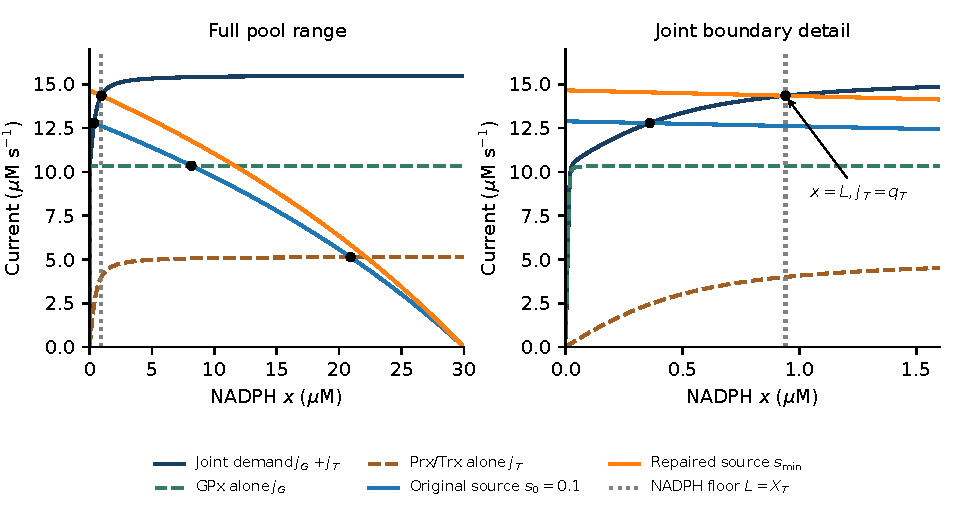
\includegraphics[width=\linewidth]{intersections.pdf}
\caption{The same kinetic laws in separate and joint preparations. Intersections of
a source curve with a demand curve determine the equilibrium NADPH concentration;
black markers show the isolated GPx, isolated Prx/Trx and joint equilibria at
$s_0=0.1$, and the joint equilibrium at $s_{\min}$. The repaired source meets the
joint demand exactly at the binding floor $L=X_T$, where the Trx current equals its
quota. Direct numerical solution of these same kinetics reproduces the boundary;
the theorem adds necessity, sufficiency, attainment and species reconstruction.}
\label{fig:intersections}
\end{figure}

\subsection{Separate success and joint failure}

At the reference setting $s_0=0.1$ the two isolated preparations deliver
$10.351411$ and $5.129763$ \fluxunit, both above their quotas; their individual
requirements are only $s=0.077641$ and $s=0.031699$. The joint preparation at the
same setting equilibrates at $x\approx0.3597903$ \uM\ with currents
$10.344228$ and $2.440510$ \fluxunit, so the Trx quota fails by a wide margin
(Figure~\ref{fig:intersections}). Both isolated successes and the joint failure
are verified in Lean.

Joint quota failure is not a statement that adding the second branch lowered
aggregate antioxidant activity. At that same setting the total counted NADPH
turnover is $j_G+j_T\approx12.784739$ \fluxunit, already larger than the GPx-only
current $10.351411$ \fluxunit, and the peroxide turnover \eqref{eq:peroxide} is
larger still. What fails is the specified pair of branch-resolved requirements.

\subsection{Repair decisions and the overdelivery penalty}

\begin{table}[tb]
\centering\small
\caption{Repair decisions for the declared preparation. Capacity is $sV$, not
realized steady flux; the realized demand at the boundary is
$14.348944$ \fluxunit. Decimal entries are numerical evaluations of exact
quantities, except that the fixed-kinetics minimum is additionally enclosed by
\eqref{eq:certified}.}
\label{tab:repairs}
\begin{tabular}{lrrr}
\toprule
Decision & Scale $s$ & Capacity $sV$ (\fluxunit) & Change from $s_0$\\
\midrule
Reference preparation & $0.100000000$ & $37.500000$ & $0\%$\\
Quota-only bound & $0.110947356$ & $41.605259$ & $10.947356\%$\\
Fixed-kinetics minimum $s_{\min}$ & $0.113712668$ & $42.642250$ & $13.712668\%$\\
Enzyme redesign $s^\star$ & $0.110947356$ & $41.605259$ & $10.947356\%$\\
$s_{\min}$ with $5\%$ source tolerance & $0.119697545$ & $44.886579$ & $19.697545\%$\\
Declared parameter box (Appendix~\ref{app:box}) & $0.125895729$ & $47.210898$ & $25.895729\%$\\
\bottomrule
\end{tabular}
\end{table}

Table~\ref{tab:repairs} collects the capacity decisions. The kinetic overdelivery
of Proposition~\ref{prop:overdelivery} is
$j_G(L)-q_G=0.348943552$ \fluxunit, entirely on the non-binding GPx branch. It
makes the true requirement $2.49245\%$ larger than the quota-only estimate; as
repair percentages relative to $s_0$, the two differ by $2.76531$ percentage
points. This is an identified kinetic effect with a closed-form value, not an
unexplained discrepancy between two numerical procedures.

The redesign of Section~\ref{sec:redesign} takes the larger root of
\eqref{eq:redesign}, $g^\star\approx361.3505536$ \uM, giving
\[
  E_G^\star\approx48.313664\ \uM,
\]
a $3.37267\%$ reduction of the GPx pool. Both currents then sit exactly at quota
and the quota-only bound is attained. The smaller root of \eqref{eq:redesign} is
rejected: it would require an enzyme pool of about $9.07\times10^4$ \uM. Even the
optimal reallocation still needs more regeneration than the reference setting,
$s^\star\approx0.110947>0.1$; that this cannot be evaded by any admitted redesign
of the glutathione branch is Proposition~\ref{prop:lower}, and it is verified in
Lean for the nominal instance.

\begin{table}[tb]
\centering\small
\caption{The reconstructed steady state at the attained minimum
$s=s_{\min}$, $x=L=X_T$. All four conservation laws and all reaction balances hold;
the displayed digits are rounded evaluations, not the exact certificates.}
\label{tab:boundary}
\begin{tabular}{lr@{\qquad}lr}
\toprule
Species & Value (\uM) & Species & Value (\uM)\\
\midrule
NADPH $x$              & $0.940319216$  & Reduced Trx $y$        & $0.217306271$\\
NADP$^+$ $P-x$         & $29.359680784$ & Oxidized Trx $z_T$     & $0.287693729$\\
Free GSH $g$           & $361.118523602$& Reduced Prx $r$        & $10.000000000$\\
GSSG $z$               & $5.219305298$  & Sulfenic Prx $h$       & $0.266666667$\\
Reduced GPx $e_0$      & $49.280683581$ & Hyperoxidized Prx $w$  & $0.064000000$\\
Oxidized GPx $e_1$     & $0.716450616$  & Disulfide Prx $v$      & $8.765333333$\\
GPx--SSG $e_2$         & $0.002865802$  & & \\
\bottomrule
\end{tabular}
\end{table}

\subsection{Ceilings and the narrow binding interval}

\begin{figure}[tb]
\centering
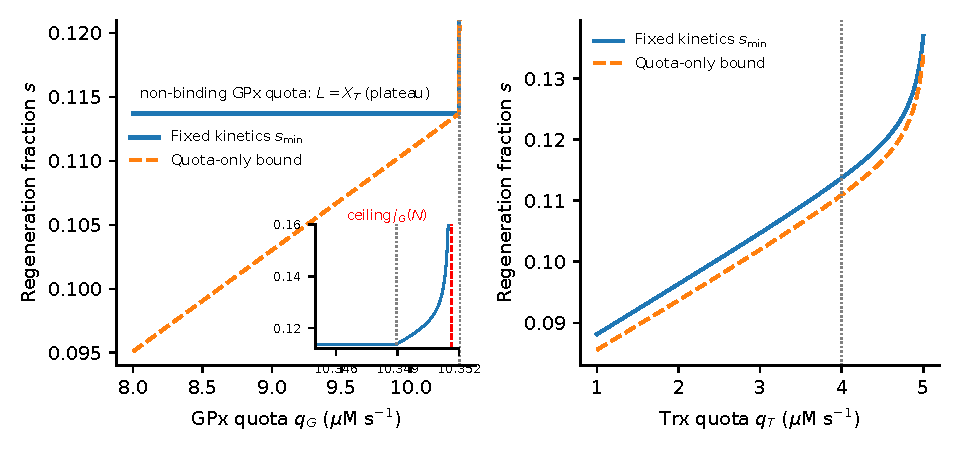
\includegraphics[width=\linewidth]{quotas.pdf}
\caption{Required regeneration as one quota varies with the other held at its
nominal value. Left: over most of the displayed range the GPx quota is non-binding,
$L=X_T$, and the fixed-kinetics minimum is exactly constant, while the quota-only
bound decreases spuriously; the dotted line marks the switching quota
$q_G=j_G(X_T)$, and the inset resolves the narrow interval between that switch and
the ceiling $j_G(N)$, where the requirement diverges. Right: raising the Trx quota
raises its NADPH floor and hence the requirement. Dashed curves omit kinetic
overdelivery.}
\label{fig:quotas}
\end{figure}

The branch ceiling currents of Theorem~\ref{thm:ceiling} are
\[
  j_G(N)\approx10.351642\ \fluxunit,\qquad j_T(N)\approx5.143547\ \fluxunit .
\]
Both nominal quotas lie strictly below them, so a finite repair exists; this
instance of Theorem~\ref{thm:ceiling} is verified in Lean. Quotas at or above
these values are unattainable at any finite capacity.

Figure~\ref{fig:quotas} shows the resulting quota dependence. Lowering the GPx
quota leaves $s_{\min}$ exactly unchanged over the non-binding plateau, while the
quota-only line falls, which is the graphical form of
Proposition~\ref{prop:overdelivery}. The plateau ends at the switching quota
$q_G=j_G(X_T)=10.348944$ \fluxunit, above which the GPx branch binds; the interval
between that switch and the ceiling $10.351642$ \fluxunit\ has width only
$0.0027$ \fluxunit, which is why it needs an inset rather than a shared axis. Both
values must be labelled separately, and neither should be rounded onto the other.

\section{How far the criterion extends}\label{sec:scope}

Theorem~\ref{thm:main} uses far less than the specific rate laws of
Section~\ref{sec:model}. This section states what it actually needs, and what
replaces it when those hypotheses fail. The results here are conventional
mathematics; they are not part of the formalized development.

\subsection{Any strictly decreasing source}\label{sec:general}

The proof of Theorem~\ref{thm:main} uses only that $x\mapsto R_s(x)=s\,r(x)$ is
continuous, positive on $[0,N)$, strictly decreasing, and vanishing at $N$. Hence
for any such $r$,
\begin{equation}\label{eq:general}
  s_{\min}=\frac{J(L)}{r(L)} ,
\end{equation}
with the same necessity, sufficiency and attainment. In particular, multiplying
the source by any positive nonincreasing factor preserves the theorem. Product
inhibition of the regenerating enzyme by NADPH is of this type: for illustration,
$r(x)\mapsto r(x)/(1+x/K_I)$ is admissible for every $K_I>0$. We stress that this
is a mathematical illustration, not a fitted mechanism for a particular
dehydrogenase; a quantitative claim would require the mechanism and assay
conditions of the enzyme in question \citep{adediran1991,stanton2012}.

\subsection{More than two branches}

For finitely many branches with private states, each with a continuous strictly
increasing service current, coupled only through one decreasing source, the proof
is unchanged:
\[
  L=\max_iX_i,\qquad J=\sum_ij_i,\qquad s_{\min}=\frac{J(L)}{r(L)},
\]
and the overhead is $\sum_i\bigl[j_i(L)-q_i\bigr]/r(L)$. This covers additional
independent NADPH sinks, but not shared private carriers, competing binding sites,
several independent cofactors, or cross-inhibition; those require first reducing
the enlarged state equations with the same properties.

\subsection{Carrier floors and redox endpoints}\label{sec:floors}

Service quotas can be restated in the variables that are actually measured. By
\eqref{eq:inversion} the quota $j_i\ge q_i$ is exactly the carrier floor
$u_i\ge Y_i$, and conversely a desired free-GSH floor $g\ge g_{\mathrm{req}}$ within
the attainable pool range corresponds to
\[
  q_G=\frac{E_Ga_G\,g_{\mathrm{req}}}{g_{\mathrm{req}}+\rho_G} .
\]
This is a steady-state equivalence; it does not equate instantaneous oxidative and
reductase currents during transients.

Ratio endpoints can be treated the same way, with care about conventions. At fixed
temperature $\Theta$, pH and a declared activity convention, the formal half-cell
potentials are
\begin{equation}\label{eq:nernst}
  \mathcal E_G=\mathcal E_G^{\circ\prime}
    +\frac{R\Theta}{2F}\ln\frac{a_{\mathrm{GSSG}}}{a_{\mathrm{GSH}}^2},
  \qquad
  \mathcal E_T=\mathcal E_T^{\circ\prime}
    +\frac{R\Theta}{2F}\ln\frac{a_{\mathrm{Trx,ox}}}{a_{\mathrm{Trx,red}}} ,
\end{equation}
with dimensionless activities \citep{schafer2001}. Inserting bare micromolar
numbers into the glutathione logarithm silently changes the standard state and
gives an incorrect absolute potential; only $a=c/c^\circ$ with an explicit
$c^\circ$ is meaningful. For thioredoxin, $z_T=T-y$, so a specification
$\mathcal E_T\le\mathcal E_{T,\mathrm{target}}$ is equivalent to the carrier floor
\[
  y\ \ge\ \frac{T}{1+\exp\bigl[2F(\mathcal E_{T,\mathrm{target}}
    -\mathcal E_T^{\circ\prime})/(R\Theta)\bigr]} ,
\]
which enters the same threshold inversion provided it lies in the attainable
range. Specifying a favourable potential does not create carrier capacity.

For glutathione, use the \emph{free} $g$ and $z$, retaining bound material only in
the conservation law. At steady state, with $C_0=E_Ga_G/c_G$,
\[
  z(g)=\tfrac12\left(G-g-\frac{C_0}{g+\rho_G}\right),
  \qquad
  \frac{\dd z}{\dd g}=\tfrac12\left[-1+\frac{C_0}{(g+\rho_G)^2}\right],
\]
so $C_0\le\rho_G^2$ is a simple sufficient condition for $z$ to be nonincreasing in
$g$. It holds nominally, with $C_0=1.05$ and $\rho_G^2=27.783441$ $\uM^2$. Since
$g$ increases with $x$ and $z>0$, the ratio $z/g^2$ then strictly decreases, so a
feasible upper bound on $\mathcal E_G$ also supplies a lower NADPH threshold and
can be used in place of a flux quota. This route translates assay specifications
into endpoints without importing a generic ``healthy potential''; it supplies no
standard potentials and no medically meaningful targets, and a Nernst readout does
not certify the thermodynamic consistency of an irreversible rate law.

\subsection{Non-monotone branch service}\label{sec:nonmono}

Monotonicity of $j_i$ belongs to the mechanism of Section~\ref{sec:model}. Other
mechanisms need not have it: the mechanistic thioredoxin-system model of
\citet{pannala2015} includes NADPH substrate inhibition, which can make a branch
current non-monotone in $x$. Substrate inhibition inside a consuming branch is a
different matter from product inhibition of the source, and cannot be handled by
\eqref{eq:general}.

What survives is an exact characterization rather than a threshold. Suppose the
private states remain uniquely reconstructible for each $x$ and $r>0$ on $(0,N)$.
Put
\begin{equation}\label{eq:intervals}
  \mathcal K=\{x\in(0,N):\ j_i(x)\ge q_i\ \text{for all } i\},
  \qquad h(x)=\frac{J(x)}{r(x)} .
\end{equation}
Then the set of scales admitting a successful steady state is exactly
$\mathcal S=h(\mathcal K)$. For a closed component $[\alpha,\beta]$ of
$\mathcal K$ on which $h$ is continuous and increasing, the contribution is
$[h(\alpha),h(\beta)]$; endpoint inclusion must be handled explicitly for open
components. Equivalently, on an interval where $F_s$ is strictly decreasing, a root
in $[\alpha,\beta]$ exists exactly when $F_s(\alpha)\ge0\ge F_s(\beta)$ --- which
proves a statement on that interval without excluding roots outside it. Turning
this into a decision procedure requires certifying the quota crossings and turning
points and bounding $h$ on each monotone piece.

Two conclusions that are sometimes drawn from non-monotonicity do not follow. The
first is that the equilibrium must become non-unique; the second is that excess
regeneration must be harmless. The following example refutes both simultaneously.

\begin{example}[Excess regeneration destroys service without bistability]
\label{ex:counter}
Take the dimensionless system on $0<x<1$ with
\[
  r(x)=1-x,\qquad j(x)=x\left(\tfrac65-x\right),\qquad q=\tfrac3{10} .
\]
The current increases up to $x=3/5$ and decreases thereafter, so it is not
monotone. Nevertheless
\[
  h(x)=\frac{x(6/5-x)}{1-x},\qquad
  h'(x)=\frac{(1-x)^2+1/5}{(1-x)^2}>0 ,
\]
and $h$ maps $(0,1)$ onto $(0,\infty)$, so there is exactly one positive
equilibrium for every $s>0$ and no bistability. The quota holds exactly on
$\bigl[\tfrac{6-\sqrt6}{10},\tfrac{6+\sqrt6}{10}\bigr]$, equivalently for
\[
  \frac{12-3\sqrt6}{10}\ \le\ s\ \le\ \frac{12+3\sqrt6}{10},
  \qquad\text{numerically } 0.465153\le s\le1.934847 .
\]
Thus service has an \emph{upper} operating limit as well as a lower one. In the
scalar dynamics $\dot x=s\,r(x)-j(x)$ the derivative at equilibrium is
$-r(x)h'(x)<0$, so the example is also locally stable throughout.
\end{example}

Bistability requires multiple stable states and appropriate dynamics; a candidate
steady-state fold needs $F_s=0$ and $\partial F_s/\partial x=0$ together with a
nondegeneracy condition. Non-monotone kinetics alone imply none of this. Note also
that monotonicity of each individual branch is sufficient but not necessary for
the criterion: what the argument requires is only $F_s'<0$, which a non-monotone
$j_i$ need not violate.

\section{Full dynamics: what follows and what does not}\label{sec:dynamics}

\begin{figure}[tb]
\centering
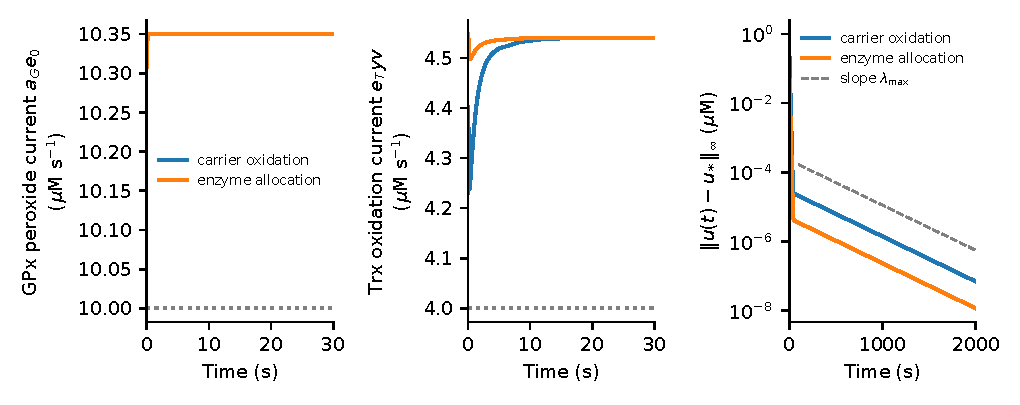
\includegraphics[width=\linewidth]{transients.pdf}
\caption{Full-state perturbations at $s=0.12$, a setting with strict service slack,
with initial conditions defined in Appendix~\ref{app:ode}. Left and centre: the
peroxide and oxidation currents recover within a few seconds and stay above their
quotas (dotted lines) from the first sample. Right: the same trajectories over the
full $2000$ s integration, measured as the infinity-norm distance to the
equilibrium on a logarithmic scale; the grey reference line has the slope of the
slowest Jacobian eigenvalue, $-0.0030043$ s$^{-1}$. Rapid recovery of the plotted
currents and slow relaxation of the full state are different statements.}
\label{fig:transients}
\end{figure}

After eliminating the four conserved totals, the maintained system has eight
independent variables; Appendix~\ref{app:ode} gives the equations, the admitted
domain and the numerical protocol.

\paragraph{Forward invariance.}
The physically admitted closed domain
\[
  0\le x\le N,\quad z\ge z_{G0},\quad z_T\ge z_{T0},\quad
  g,e_0,e_1,e_2,y,r,h,w,v\ge0
\]
is forward invariant, by the inward boundary inequalities collected in
Appendix~\ref{app:ode}. In particular the baseline-subtracted reductase laws never
produce a negative current on this domain, and its compactness excludes finite-time
escape. This is a direction-consistency check, not a free-energy realization of
the phenomenological model. Neither boundedness nor uniqueness of the equilibrium
implies global convergence.

\paragraph{Numerical evidence.}
At $s=0.1$, $s=s_{\min}$ and $s=0.12$ the reconstructed equilibria have residuals
below $10^{-12}$ \fluxunit\ and Jacobians whose largest eigenvalue real parts are
\[
  -0.002999934,\qquad -0.003001207,\qquad -0.003004280\ \ \mathrm{s}^{-1},
\]
so each is numerically locally stable. The corresponding slow modal time scale is
about $333$ s. Two perturbations were applied at each setting, one oxidizing the
carriers and one redistributing enzyme states within their conserved totals. At
$s=0.12$ both trajectories keep both service currents above quota from the first
sample; at $s=0.1$ neither attains joint service; at the exact boundary
$s=s_{\min}$, where the limiting service margin is zero, both transiently violate
the Trx quota, with sampled minima $3.631856$ and $3.944233$ \fluxunit, and
apparent permanent passage only near $51.55$ s. At zero limiting margin such a
sampled crossing time is not a certified guarantee, and we do not report it as one.
The late-time decay of the full-state error matches the slow eigenvalue to five
significant figures (Figure~\ref{fig:transients}, right panel), which is a
consistency check on the linearization rather than an independent stability proof.

\paragraph{A monotone-systems shortcut is unavailable.}
It is tempting to hope that the eight-variable system is cooperative in some
orthant order, which would bring the theory of monotone systems to bear
\citep{hirsch1985,smith1995,angeli2003}. It is not. In the reduced coordinates of
Appendix~\ref{app:ode},
\begin{equation}\label{eq:coop}
  \frac{\partial\dot e_1}{\partial e_2}=-a_G+b_Ge_1,
  \qquad
  \frac{\partial\dot e_2}{\partial e_1}=b_Gg ,
\end{equation}
which at the nominal boundary equilibrium take the values $-0.181341975$ and
$14.444740944$ $\mathrm{s}^{-1}$. Their signs are not a floating-point artefact:
at steady state $b_Ge_1=j_G/g=a_Ge_0/g<a_G$ because $e_0\le E_G=50$ while
$g>361$, so the first entry is strictly negative and the second strictly positive.
A diagonal sign change $\sigma_i\in\{\pm1\}$ leaves the product of the two
transposed off-diagonal entries unchanged, whereas a cooperative Jacobian would
have both nonnegative and hence a nonnegative product. Therefore \emph{no} fixed
orthant sign transformation makes this system cooperative near the boundary
equilibrium. This does not exclude a more general cone, other coordinates, or a
different stability proof; it does exclude treating the standard hypotheses as
already satisfied. For the same reason, deficiency-based results
\citep{feinberg1987} cannot be invoked by naming the framework alone: the
saturating source and baseline-corrected laws would first have to be given an
explicit reaction realization and kinetic class.

\paragraph{What a genuine certificate would require.}
A local certificate at a point with strict slack, say $s=0.12$, is the economical
next step: enclose the equilibrium with rational bounds keeping strict service
margins, rationalize a Lyapunov matrix $P$ for the enclosed linearization, certify
$P\succ0$ and $A^{\!\top}P+PA\preceq-\alpha I$, bound the nonlinear remainder by
$C\|\xi\|^2$ on an explicit neighbourhood, and choose an ellipsoid on which the
cubic term is dominated. A numerical Lyapunov matrix by itself is not that
certificate, and none is claimed here. This is optional for a steady-state result
and we do not make the present conclusions depend on it.

\begin{table}[tb]
\centering\small
\caption{Maintained-input and material accounting for the declared subsystem.}
\label{tab:accounting}
\begin{tabular}{p{0.24\linewidth}p{0.70\linewidth}}
\toprule
Feature & Accounting and scope\\
\midrule
Peroxide clamp & An external feed balances \eqref{eq:peroxide}; the challenge is a
clamp, not a finite bolus. At the boundary the declared inventory-to-turnover ratio
is $H/I_H\approx7.0\times10^{-4}$ s, so the clamp and mixing assumptions need
explicit experimental attention.\\
NADPH regeneration & $P$ is conserved and $P_0$ is a baseline offset. The product
$sV$ scales an externally driven source whose substrate supply and work are not
state variables of the model.\\
Prx maintenance & At the boundary the repair current is
$c_Tw=b_Tj_T/d_T=0.000192$ \fluxunit. It is an external input, not free reducing
power, and its ATP and thiol requirements are not resolved
\citep{jonsson2008}.\\
Private inventories & The glutathione total includes GPx-bound material; Trx and
both enzyme totals are conserved. The redesign changes only the declared GPx
inventory, keeping all carrier totals fixed.\\
Removed pathways & Protein-thiol reactions, catalase, transport, synthesis and
efflux are absent from the selected subsystem. Their protective functions and
resource demands cannot be inferred from these results.\\
\bottomrule
\end{tabular}
\end{table}

Because no complete set of reversible rate constants, chemical potentials or
chemostat work is specified, a claim of thermodynamic incompatibility would be
unsupported, and none is made. Table~\ref{tab:accounting} records what each
maintained input is and is not.

\section{Relation to existing methods, and a discriminating experiment}
\label{sec:relation}

Direct numerical solution of the same kinetic model produces the same equilibria.
It is a matched computational baseline, not a competing prediction. What the exact
analysis adds is the decision inequality itself, the attainment of the boundary,
the impossibility statement below it, uniqueness of the full state, the ceiling
equivalence, and the closed-form separation of the three interventions. A
simulation alone cannot supply an impossibility certificate.

Thermodynamics-based metabolic flux analysis constrains flux and metabolite
activity profiles by thermodynamic feasibility \citep{henry2007}. That addresses a
different question from satisfying fixed kinetic branch requirements at one shared
concentration in a maintained preparation, and we make no claim to supersede it.
Enzyme cost minimization computes enzyme allocations supporting specified fluxes
under kinetic and thermodynamic constraints \citep{noor2016}. Our fixed-enzyme
theorem holds enzyme pools fixed, while \eqref{eq:redesign} permits exactly one
declared design variable and gives a closed-form optimum with a matching lower
bound for it; this is narrower than, and not a replacement for, a general
allocation framework. Nor is resource competition for NADPH itself a new
observation \citep{stanton2012,fan2014}; the contribution here is the exact
decision and reconstruction theorem for a declared retained-state model.

A discriminating experiment fixes enzyme amounts, carrier inventories and peroxide
conditions, estimates the kinetic parameters and the source response \emph{once}
with uncertainty, and then varies regeneration through the precomputed boundary
without refitting at each setting. Measurements should resolve NADPH together with
branch-resolved turnover or reduced-carrier states, since total NADPH consumption
or total peroxide clearance alone does not identify the two branch currents.
Useful controls are distinct: removing a branch, relaxing a quota (which is a
reporting control only, since it changes no trajectory), and the controlled change
of GPx abundance. For the redesign, compare the original and redesigned
preparations both at their respective required capacities and at a common
capacity, and report service margins and total peroxide turnover separately: an
allocation that is optimal for meeting quotas will deliberately reduce turnover
above them.

The immediate application setting is a maintained reconstituted or cell-free
multienzyme preparation, where independent branch requirements can represent
minimum reporter turnover or the preservation of two reduced-carrier pools. This
is a proposed application of the model, not a report that such a preparation has
been built: the clamp, the baseline-subtracted reductase laws, the conserved pools
and the external repair step all still require an implementation or a justified
operating approximation. A living-cell interpretation would additionally require
transport, alternative clearance, competing NADPH uses, regulation, and justified
functional endpoints. Full reproduction of the published cellular time courses and
an empirical uncertainty calibration remain separate tasks, and nothing here is a
clinical intervention.

\paragraph{Reproducibility.}
All constants printed in this paper are recomputed from the model definition by a
single replay script, which checks the exact rational thresholds and enclosures,
every table entry, the Jacobian spectra, the transient minima and the parameter-box
arithmetic. \RepositoryNote

\appendix

\section{Full maintained ODE and numerical protocol}\label{app:ode}

Use coordinates $u=(x,z,e_1,e_2,z_T,h,w,v)$ and recover the eliminated variables
from the conservation laws,
\[
  g=G-2z-e_2,\qquad e_0=E_G-e_1-e_2,\qquad y=T-z_T,\qquad r=E_T-h-w-v .
\]
Write the glutathione currents as
$\Phi_0=a_Ge_0$, $\Phi_1=b_Gge_1$, $\Phi_2=c_Gge_2$, $\Psi_G=k_Gx(z-z_{G0})$, and
the peroxiredoxin--thioredoxin currents as
$\Theta_r=a_Tr$, $\Theta_w=b_Th$, $\Theta_h=c_Tw$, $\Theta_v=d_Th$,
$\Theta_y=e_Tyv$, $\Psi_T=k_Tx(z_T-z_{T0})$. The system is
\begin{equation}\label{eq:ode}
\begin{aligned}
  (\dot x,\dot z,\dot e_1,\dot e_2)
    &=\bigl(\,R_s(x)-\Psi_G-\Psi_T,\ \ \Phi_2-\Psi_G,\ \ \Phi_0-\Phi_1,\ \
      \Phi_1-\Phi_2\,\bigr),\\
  (\dot z_T,\dot h,\dot w,\dot v)
    &=\bigl(\,\Theta_y-\Psi_T,\ \
      \Theta_r+\Theta_h-\Theta_w-\Theta_v,\ \ \Theta_w-\Theta_h,\ \
      \Theta_v-\Theta_y\,\bigr).
\end{aligned}
\end{equation}

\paragraph{Forward invariance.}
On the admitted domain of Section~\ref{sec:dynamics} the vector field points
inward at every face. At $x=0$ both reductase currents vanish and
$\dot x=R_s(0)>0$; at $x=N$ regeneration vanishes and $\dot x=-\Psi_G-\Psi_T\le0$.
At $z=z_{G0}$ and $z_T=z_{T0}$ the derivatives are $\Phi_2\ge0$ and
$\Theta_y\ge0$. At $g=0$ we get $\dot g=-\Phi_1-\Phi_2+2\Psi_G=2\Psi_G\ge0$, and
at $y=0$, $\dot y=\Psi_T\ge0$. Every zero enzyme state has nonnegative production:
in particular $\dot e_0=\Phi_2-\Phi_0$, $\dot e_1=\Phi_0-\Phi_1$,
$\dot e_2=\Phi_1-\Phi_2$, $\dot r=\Theta_y-\Theta_r$ and $\dot w=\Theta_w-\Theta_h$
are nonnegative when the respective variable vanishes. The source denominator stays
positive because $D>N$. These inequalities with local smoothness give invariance of
the conserved polytope. This is a conventional ODE argument and is not part of the
formalized development.

\paragraph{Numerical protocol.}
Equilibria were located by scalar bracketing of $F_s$ followed by full-state
reconstruction through \eqref{eq:greconstruct}--\eqref{eq:treconstruct}, giving
residuals below $10^{-12}$ \fluxunit. Jacobians were formed by complex-step
differentiation with step $10^{-20}$, which is free of subtractive cancellation.
Integrations used an implicit Radau method with relative tolerance
$2\times10^{-9}$ and absolute tolerance $2\times10^{-11}$ over $2000$ s, sampled
densely over the first $5$ s and then every $3.325$ s. The carrier-oxidation
perturbation increases $z$ by $1$ \uM\ and $z_T$ by $0.02$ \uM; the
enzyme-allocation perturbation increases $e_1$ by $0.2$ \uM\ and $h$ by
$0.05$ \uM. Both start strictly inside the admitted domain, and every sampled
state remained in it. Final infinity-norm distances to the equilibria were below
$1.2\times10^{-7}$ \uM.

At $s=0.12$ the smallest sampled service currents are $(10.349641,4.231028)$ for
carrier oxidation and $(10.308165,4.497447)$ \fluxunit\ for enzyme
redistribution, both above quota from the first sample. At $s=s_{\min}$ the
respective minimum Trx currents are $3.631856$ and $3.944233$ \fluxunit, below
quota, as discussed in Section~\ref{sec:dynamics}. Sampling and solver tolerances
do not by themselves certify an inequality between samples.

\section{A conservative declared parameter box}\label{app:box}

To separate operating tolerance (Section~\ref{sec:tolerance}) from parameter
uncertainty, consider an explicit design box in which $E_G$ and $E_T$ vary
independently by $\pm1\%$ and $k_G$ and $k_T$ independently by $\pm5\%$, all other
quantities fixed. These intervals are declared assumptions, not estimated
biological ranges. All inequalities below are evaluated as exact fractions.

For either branch bound $Y_i$ of \eqref{eq:thresholds} by $[Y_i^-,Y_i^+]$. Both
nominal coefficients $B_i$ are negative and fixed over this box, so
\[
  \Delta_i^-=\Gm_i^--A_i(Y_i^+)^2-B_iY_i^-
\]
is a valid lower bound for $\Delta_i$; when it is positive,
$X_i\le C_i^+Y_i^+/\Delta_i^-$. The glutathione constant uses
$\Gm_G^-=S_G\rho_G-E_G^+a_G/c_G$, while $\Gm_T=S_T$ is fixed. This gives
\[
  X_G<0.059173\ \uM,\qquad X_T<1.062578\ \uM
\]
throughout the box. Choose the common target $x_*=1.5$ \uM, which exceeds both.
Carrier conservation gives $g\le S_G=368$ and $y\le S_T=0.43$, so monotonicity of
the rational currents in \eqref{eq:flux} gives
\[
  J(x_*)\ \le\ \frac{E_G^+a_GS_G}{S_G+\rho_G}+\frac{E_T^+e_TS_T}{1+\rho_Te_TS_T}
  \ <\ 15.681942\ \fluxunit .
\]
Using the exact upper expression, its ratio to $R_1(x_*)$ is the exact rational
\begin{equation}\label{eq:sbox}
  s_{\mathrm{box}}=\frac{11621793767394811}{92312851976765625}\approx0.125895729 .
\end{equation}
At this scale the shared residual is nonnegative at $x_*$ for every admitted
parameter choice, and negative at $N$; the decreasing-residual argument then gives
a successful equilibrium at or above $x_*$. Hence $s_{\mathrm{box}}$ is sufficient
throughout the box. No optimality, corner extremality or empirical confidence is
asserted: the bound is deliberately conservative, and it does not assume that the
worst case occurs at a corner. If this box and an independent $5\%$ source
tolerance are both required, a sufficient command is $s_{\mathrm{box}}/0.95$; the
separate rows of Table~\ref{tab:repairs} are not automatically simultaneous
guarantees.

\section{Formal verification: scope and declaration map}\label{app:formal}

\subsection{Scope}

The central mathematical statements of this paper are machine-checked in
Lean~4 \citep{moura2021} against a pinned Mathlib \citep{mathlib2020}, with
warnings treated as errors. The authenticated declarations use only the standard
axioms \texttt{Classical.choice}, \texttt{Quot.sound} and \texttt{propext}; no
admitted theorem, numerical oracle, or native-computation certificate is used for
the root theorem, the nominal instance, or the redesign. The root theorem
reconstructs literal positive enzyme and carrier states, and does not assume an
equilibrium witness.

Formal checking establishes that the stated propositions follow from their stated
hypotheses. It does not eliminate the possibility of error in selecting the
equations, transcribing the source model, choosing units, or interpreting a
theorem biologically. The precise claim is that the listed declarations were kernel
checked under their stated assumptions --- not that the modelling is thereby
validated. Table~\ref{tab:evidence} classifies every substantive claim of the paper
by its actual evidence.

\begin{table}[tb]
\centering\small
\caption{Evidence class for each substantive claim.}
\label{tab:evidence}
\begin{tabular}{p{0.44\linewidth}p{0.18\linewidth}p{0.30\linewidth}}
\toprule
Claim & Evidence & Location\\
\midrule
Private-state elimination and reconstruction & Lean & Prop.~\ref{prop:elimination}\\
Continuity, monotonicity, threshold inversion & Lean & Prop.~\ref{prop:threshold}\\
Explicit derivative formulas \eqref{eq:uprime} & Conventional & Prop.~\ref{prop:threshold}\\
Sharp joint criterion, attainment & Lean & Thm.~\ref{thm:main}\\
Uniqueness of the full joint steady state & Lean & Thm.~\ref{thm:unique}\\
Separate success, joint failure at $s_0$ & Lean & Sec.~\ref{sec:nominal}\\
Certified enclosure of $s_{\min}$ & Lean & Eq.~\eqref{eq:certified}\\
Overdelivery identity, sign, equality case & Lean & Prop.~\ref{prop:overdelivery}\\
Finite-ceiling equivalence & Lean & Thm.~\ref{thm:ceiling}\\
Nominal quotas below ceilings & Lean & Sec.~\ref{sec:nominal}\\
Binding-floor identity behind the plateau & Lean & Sec.~\ref{sec:consequences}\\
Regeneration tolerance rule & Lean & Eq.~\eqref{eq:robust}\\
Redesign attainment and lower bound & Lean & Sec.~\ref{sec:redesign}\\
Reference source insufficient after any redesign & Lean & Sec.~\ref{sec:nominal}\\
Near-ceiling asymptotic cost & Conventional & Cor.~\ref{cor:asymptotic}\\
Sensitivity identities & Conventional & Eq.~\eqref{eq:sensitivity}\\
Existence of a positive equilibrium below $s_{\min}$ & Conventional & Sec.~\ref{sec:notsay}\\
General decreasing source, several branches & Conventional & Sec.~\ref{sec:scope}\\
Carrier-floor and potential translation & Conventional & Sec.~\ref{sec:floors}\\
Interval criterion and Example~\ref{ex:counter} & Conventional & Sec.~\ref{sec:nonmono}\\
Forward invariance of the admitted domain & Conventional & App.~\ref{app:ode}\\
Orthant-cooperativity obstruction & Conventional & Eq.~\eqref{eq:coop}\\
Parameter-box sufficiency & Exact rational & App.~\ref{app:box}\\
Jacobian spectra, transients, settling & Numerical & Sec.~\ref{sec:dynamics}\\
\bottomrule
\end{tabular}
\end{table}

\subsection{Declaration map}

Every name in the table below is to be read inside the single namespace
\begin{center}
\lean{CommonEnvironmentProtection}
\end{center}
and the modules are the files of that namespace. The development begins with the
quadratic-response and private-branch foundations (\lean{QuadraticPool},
\lean{PrivateBranches}); it adds the monotone-response and maintained-source
arguments (\lean{MonotoneResponse}, \lean{MaintainedSource},
\lean{CoupledPrivate}), the biochemical adapter (\lean{SourceFamilies}), the
full-state reconstruction (\lean{LiteralSteady}), the nominal instance
(\lean{SourceExample}) and the root file (\lean{Main}). The consequences,
the enzyme reallocation and the complements are in \lean{Postproof},
\lean{Allocation} and \lean{Complement}.

\begin{center}\small
\begin{tabular}{p{0.44\linewidth}p{0.50\linewidth}}
\toprule
Claim & Declaration\\
\midrule
Full joint criterion & \lean{jointProtection_iff_minimumRegeneration}\\
Failure at the reference source & \lean{source_initial_incompatible}\\
Certified repaired point & \lean{source_certified_repair}\\
Attained exact minimum & \lean{source_exact_minimum_attained}\\
Exact rational thresholds & \lean{SourceExample.exact_demand_floors}\\
Enclosure of $s_{\min}$ & \lean{SourceExample.certified_scale_bounds}\\
Both isolated preparations succeed & \lean{Postproof.isolated_successes}\\
Current equals quota at its threshold & \lean{Postproof.boundary_flux}\\
Overdelivery identity & \lean{Postproof.overdelivery_identity}\\
Overdelivery sign and equality case & \lean{Postproof.overdelivery_nonnegative}\\
Regeneration tolerance & \lean{Postproof.robust_command}\\
Binding-quota plateau & \lean{Postproof.binding_floor}\\
Ceiling obstruction & \lean{Postproof.ceiling_obstruction}\\
Redesign attainment & \lean{Allocation.allocation_attained}\\
Redesign universal lower bound & \lean{Allocation.allocation_lower_bound}\\
Reference source insufficient after redesign &
  \lean{Allocation.original_source_insufficient_for_redesign}\\
Quota below ceiling admits inversion & \lean{Complement.ceiling_admits}\\
Finite-repair equivalence & \lean{Complement.finite_repair_iff}\\
Uniqueness of the full joint state & \lean{Complement.joint_state_unique}\\
Nominal quotas below both ceilings & \lean{Complement.nominal_quotas_below_ceilings}\\
\bottomrule
\end{tabular}
\end{center}

\medskip
The exact types, hypotheses and imported axioms of these declarations, not their
names, are the authority for what has been checked. Three strict verification
receipts record the compiler invocation, the source and dependency hashes, the
exported declaration interfaces and the axiom list. The claims listed as
conventional or numerical in Table~\ref{tab:evidence} are proved or computed in
this manuscript and are deliberately not attributed to those receipts.

\bibliographystyle{plainnat}
\small
\bibliography{refs}

\end{document}
